
% ********** Chapter 5 **********
\chapter{Application Overview}
\label{sec:ApplicationOverview}

\section{Use Cases}

Web Call Example Application is a application that resides at a web server and supplies functionality of VoIP phone calls.

As shown in Figure \ref{fig:UseCasesOfWebCallExampleApplication}, there are three use cases. They are Desktop Browser, Mobile Browser and Java ME Client. This makes it possible for users to make VoIP calls anytime anywhere, to anyone. The use case of Desktop Browser is used when user have a computer connected to Internet. He can use his desktop browser, e.g. Firefox or Chrome, to access the web call site by inputing URL to address bar of browser. Users can use this web site to make VoIP phone calls as well as manage his account. The use case of Mobile Browser is just a web site for mobile browsers. The function is the same as Desktop Browser. The user can also manage his account from the Mobile Browser view. Compare with Mobile Browser, the use case of Java ME Client gives the user a even easier way to make VoIP phone calls. There is no need to sign in and input any information. As long as user pre-input everything on web site, the Java ME Client will retrieve account informations the server. All user need to do is just click the "call" button and enjoy the cheap VoIP phone calls. The Java ME Client can also load mobile phone's native contact book and call the people in the list. It can also synchronize the contact book of mobile phone to server. So user can use the contact book later when he sitting in front of a computer. A user could have multi-account for different VoIP service providers. So when the user want to make a international call, he could choose a cheap cost service provider according different rates among providers.

\begin{sidewaysfigure}
\centering
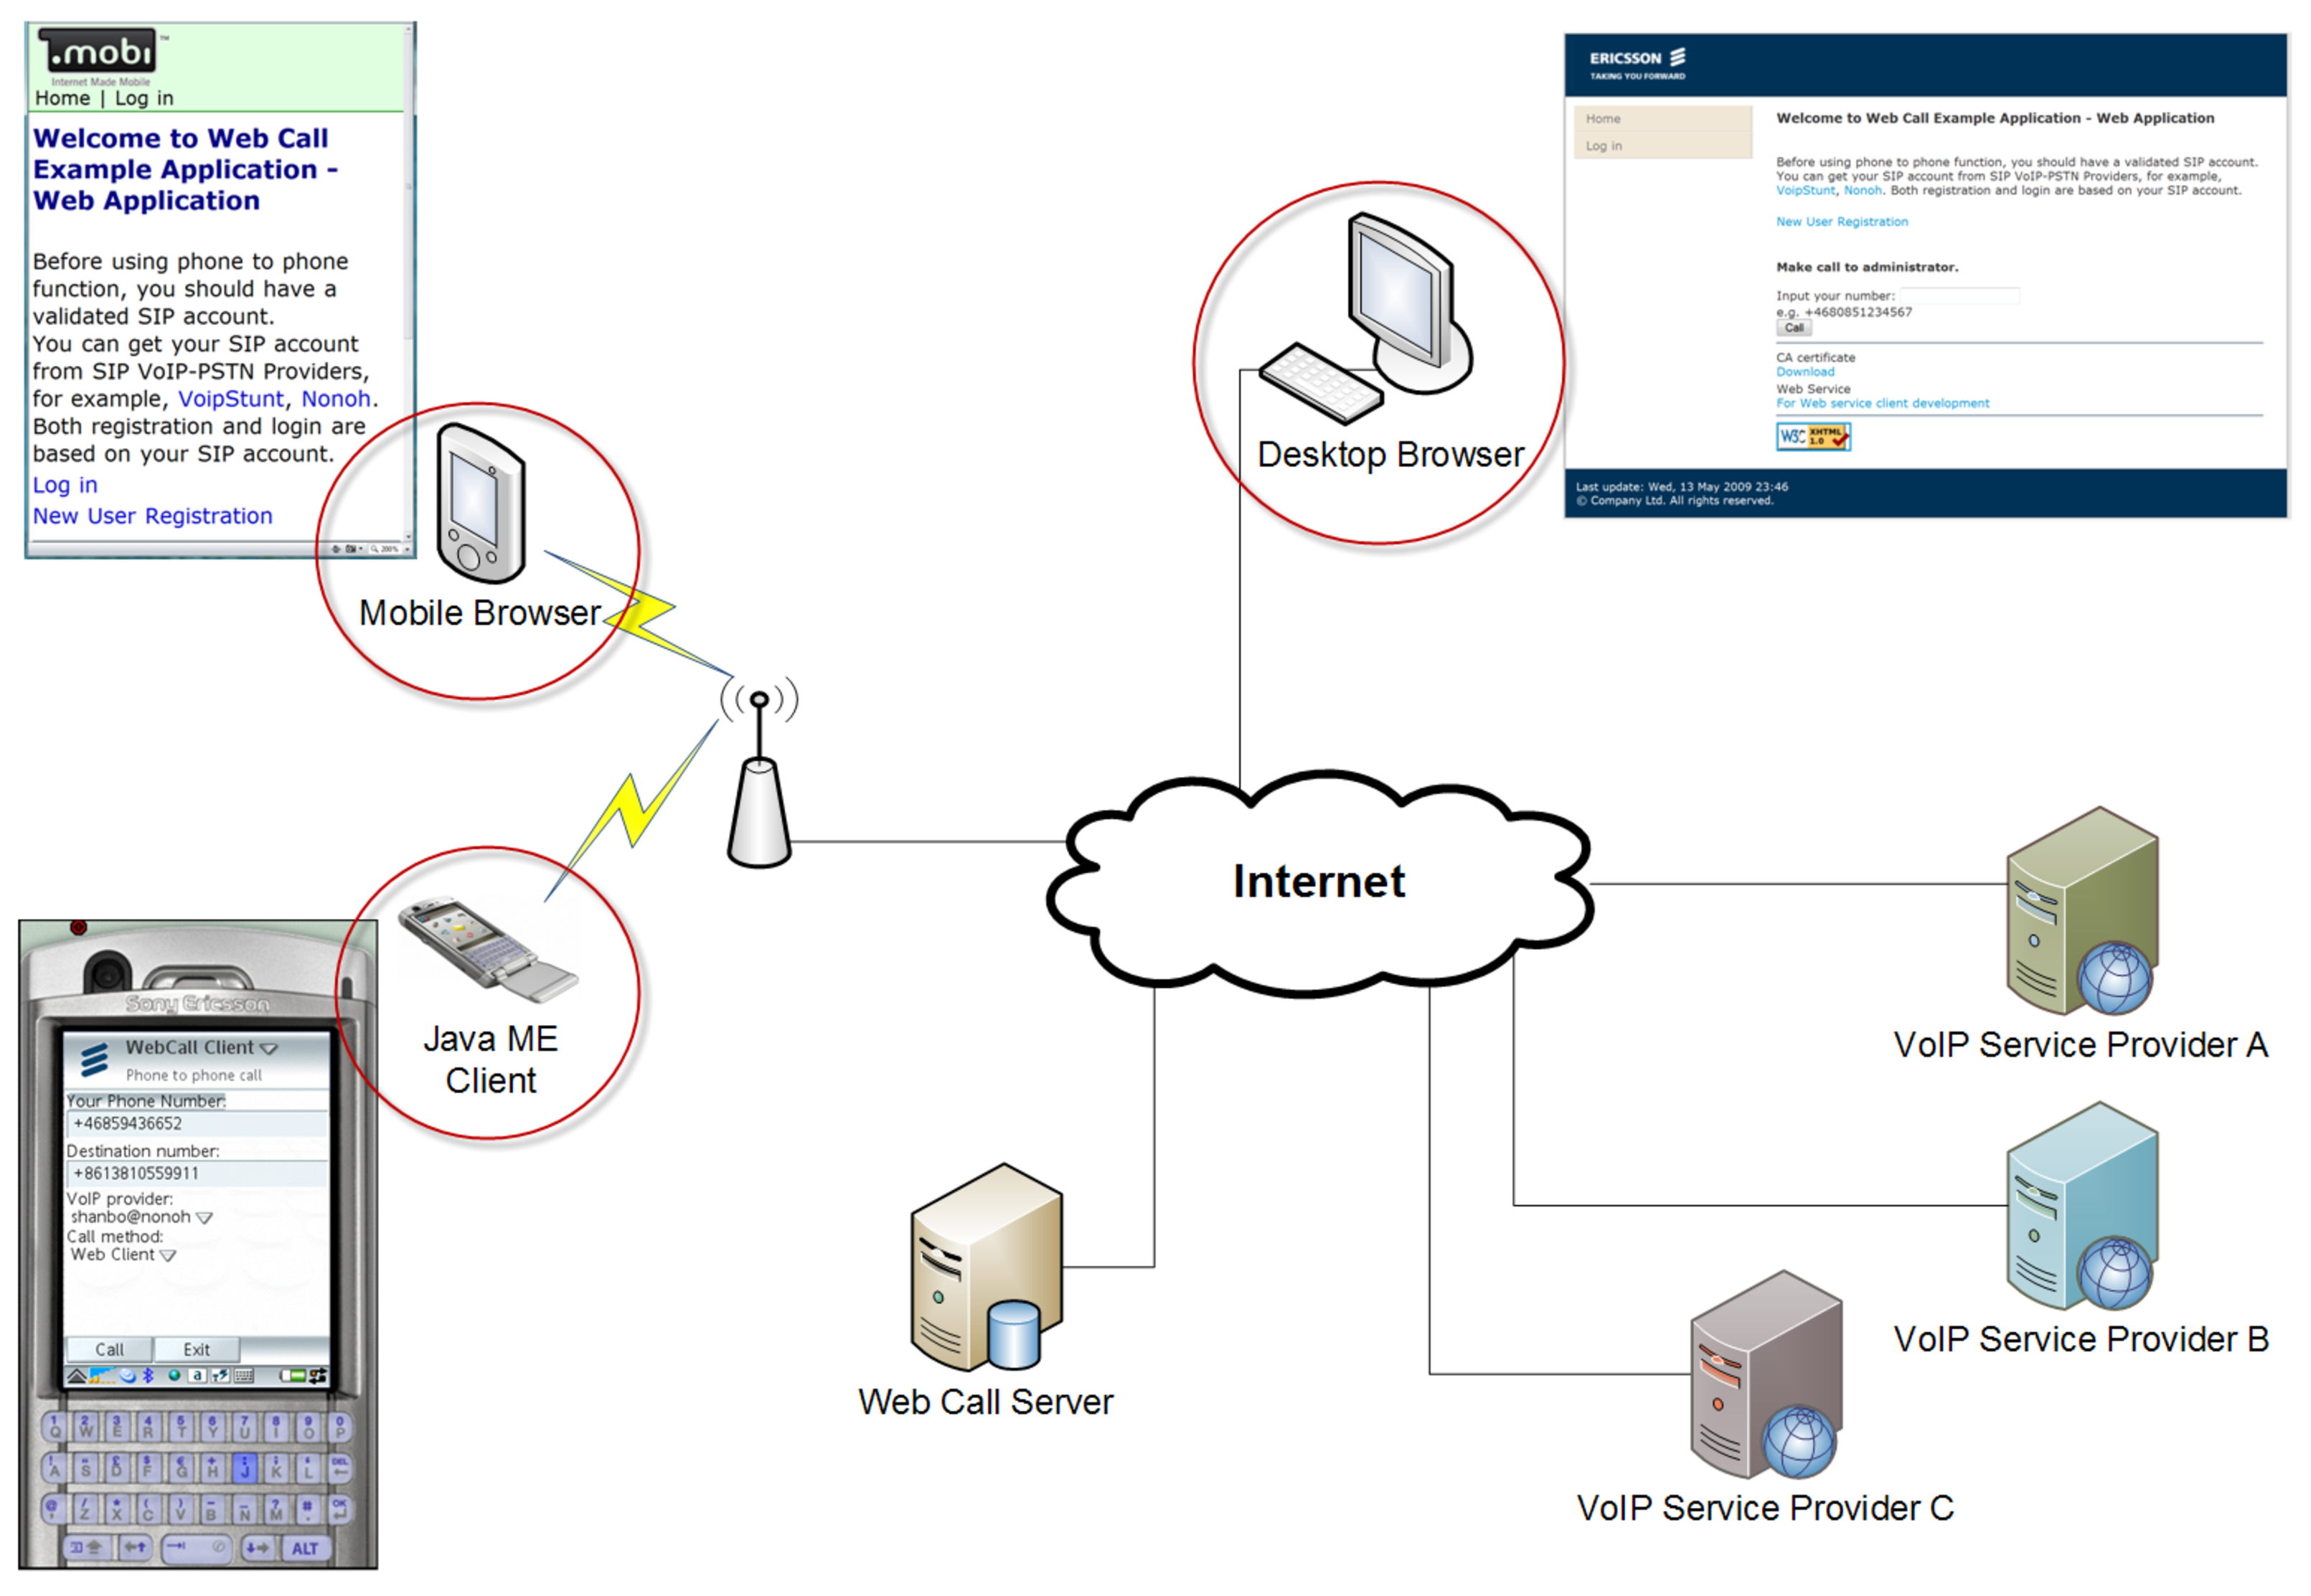
\epsfig{file=chap05/resources/use_case_overview, width=8.3in}
\caption{Use Cases of Web Call Example Application}
\label{fig:UseCasesOfWebCallExampleApplication}
\end{sidewaysfigure}


\section{Architecture}
\label{sec:ApplicationOverview:ArchitectureOverview}

This chapter presents a brief solution description of Web Call Example Application. The design architecture is shown in Figure \ref{fig:ArchitectureOfWebCallExampleApplication}.

\begin{figure}[!hbtp]
\centering
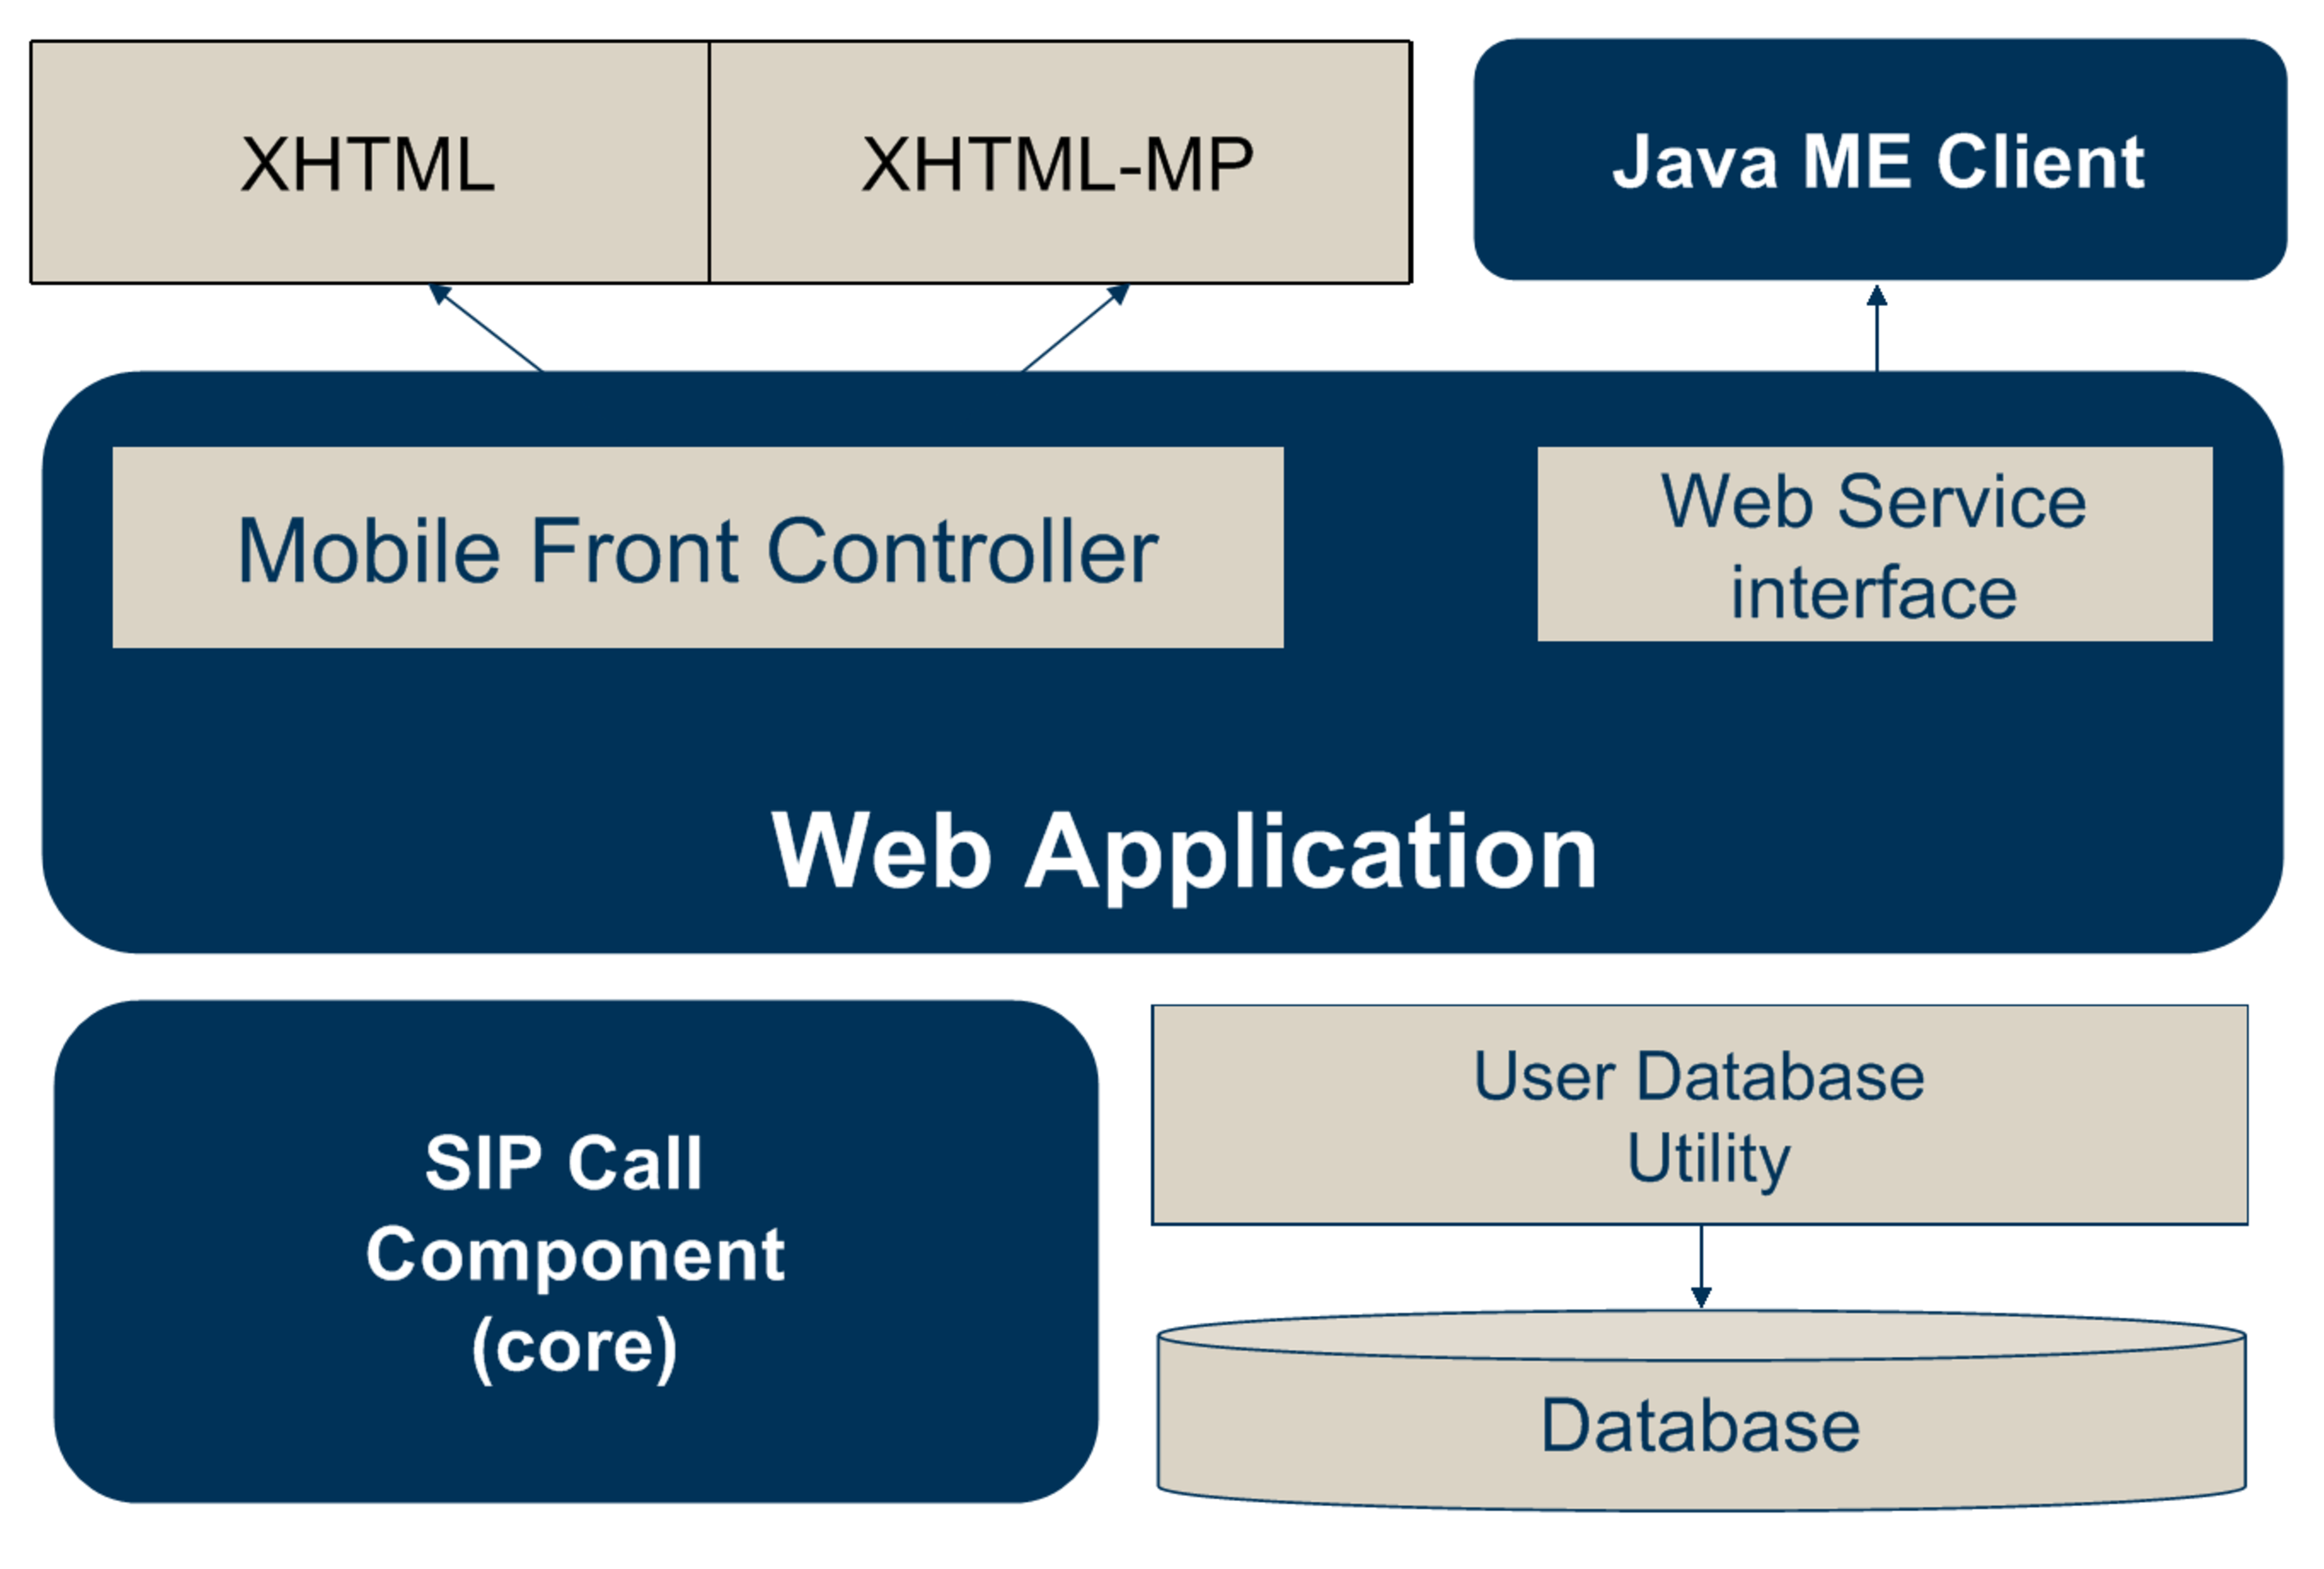
\epsfig{file=chap05/resources/architecture, width=5.2in}
\caption{The Architecture of Web Call Example Application}
\label{fig:ArchitectureOfWebCallExampleApplication}
\end{figure}

Web Call Example Application contains three components which are SIP Call Component, Web Application (include web service interface) and Java ME client. The three components are shown with dark blue back ground in Figure \ref{fig:ArchitectureOfWebCallExampleApplication}.

\subsection{SIP Call Component}

The SIP Call Component is the core of Web Call Example Application. It implemented 1 kind of relay call and four kind of third party call. It can be also used as a stand alone VoIP high-level API. 

The details about SIP Call Component will be described in Chapter \ref{sec:SIPCallComponent}.

\subsection{Web Application}

The Web Application is built on the architecture of Mobile Front Controller (MFC). SIP Call Component integrated into the web server as Java EE components: servlet, and web service. The Mobile Front Controller is used for detecting and selecting views, i.e. applications with views for desktop and mobile browsers. So Web Call Example Application supplies both XHTML view which used by desktop browser and XHTML-MP view which used by mobile browser. 

The details about Web Application will be described in Chapter \ref{sec:WebApplication}.

\subsection{Web Service Interface}

The web service interface in web application supplies a common interface for using sip call function. It uses a same database as MFC based Web Application.

The details about Web Service Interface will be described in Chapter \ref{sec:WebServiceInterface}.

\subsection{Java ME client}

Java ME client is a client of web service interface. It not only implement all of the client side function of web service interface, but also include some convenient function such as read phone contact book and synchronize with server contact book.

The details about Java ME client will be described in Chapter \ref{sec:JavaMEClient}.







% ********** End of chapter **********
